\documentclass[12pt,a4paper]{article}
\usepackage[utf8]{inputenc}
\usepackage{geometry}
\geometry{left=25mm,right=25mm,top=25mm,bottom=25mm}
\usepackage{times}
\usepackage{amsmath,amssymb}
\usepackage{graphicx}
\usepackage{caption}
\usepackage{subcaption}
\usepackage{booktabs}
\usepackage{float}
\usepackage{hyperref}
\usepackage{tikz}
\usetikzlibrary{shapes.geometric, arrows.meta, positioning}
\usepackage{pgfplots}
\pgfplotsset{compat=1.17}

\title{EMD-based Sensitive Position Analysis for Acoustic Fault Diagnosis of Air Compressors\\
\vspace{6pt}
\large A concise report based on Verma \textit{et al.}, IEEE Trans. on Reliability (2016)}
\author{Srinjoy Chakraborty (adapted notes)}
\date{\today}
\maketitle

\begin{document}
\newpage
% % TikZ styles for flowcharts
% \tikzstyle{startstop} = [rectangle, rounded corners, minimum width=3.5cm, minimum height=0.8cm,text centered, draw=black, fill=gray!10]
% \tikzstyle{process} = [rectangle, minimum width=3.5cm, minimum height=0.8cm, text centered, draw=black, fill=white]
% \tikzstyle{decision} = [diamond, aspect=2, text centered, draw=black, fill=white]
% \tikzstyle{arrow} = [->, >=Stealth]




\tableofcontents
\newpage
\begin{abstract}
Early detection of machine faults is vital to prevent costly downtime and ensure workplace safety. This paper presents a practical, data-driven process for building acoustic-based fault-diagnosis systems for reciprocating air compressors. The proposed pipeline is deliberately end-to-end: it covers how to collect acoustic data, how to choose the best microphone location using Sensitive Position Analysis (SPA), how to clean and normalize the recordings, which time/frequency/time–frequency features to extract, how to pick a compact yet informative feature set, and how to train and evaluate classifiers for multi-state fault recognition.

We validate the approach on a real single-stage reciprocating compressor with eight distinct operating states (one healthy and seven seeded faults). Using recordings from a single optimally placed microphone, the system reliably distinguishes all seeded faults; we also analyze how performance changes with different feature-selection methods, varying numbers of features, and common multiclass SVM decomposition strategies. Practical aspects—such as clipping to stable signal segments, a robust normalization routine, and the use of Empirical Mode Decomposition (EMD) to improve SPA by separating signal from noise—are emphasized so the method is applicable in noisy real-world environments.

Overall, the paper demonstrates that a carefully designed acoustic monitoring pipeline can accurately and efficiently detect multiple fault modes using only one sensor location, making the approach attractive for cost-sensitive condition-based maintenance deployments main experimental paper used as the source is \cite{Verma2016}.
\end{abstract}
\section{Introduction}
Rotating and reciprocating machines (compressors, motors, pumps) often show early warning signs in the form of acoustic or vibration signatures. Detecting faults early avoids costly downtime and safety hazards. Intelligent Condition-based monitoring (ICBM) aims to recognize incipient faults from sensory streams (acoustics, vibration, temperature, etc.) and thereby trigger maintenance before catastrophic failure. Acoustic measurements are especially attractive because they are typically easy to install and are relatively less sensitive to structural resonances compared to vibration sensors; however, acoustic recordings are often noisy and non-stationary, which makes automated analysis challenging.

Intelligent Condition-based monitoring (ICBM) is increasingly adopted in industry to detect early signs of machine degradation and to schedule maintenance before costly failures occur. Acoustic monitoring in particular is attractive for many rotating and reciprocating machines because microphones are inexpensive, simple to deploy, and can capture fault-related signatures that are often complementary to vibration and electrical measurements. However, practical acoustic monitoring faces two recurring challenges: (1) recordings are frequently contaminated by environmental and operational noise, and (2) signal characteristics are non-stationary and may vary across sensor locations. These issues make it difficult to select robust sensor placements and to extract consistently informative features for automated fault diagnosis.

A frequently overlooked but critical stage in the monitoring pipeline is \emph{Sensitive Position Analysis} (SPA) — the process of identifying where on the machine a sensor should be mounted to maximize fault detectability. Traditional SPA methods rely on straightforward statistics (e.g., RMS, peak, variance) and on simple cross-correlation to avoid redundant locations. While effective in quiet and controlled settings, these techniques can fail when recordings are influenced by heterogeneous noise or transient disturbances. To make SPA robust in such realistic settings, a preprocessing approach that can separate meaningful signal components from noise — and do so adaptively for non-stationary signals — is required.

This study proposes an end-to-end, data-driven pipeline that addresses these challenges. The core idea is to combine Empirical Mode Decomposition (EMD) with conventional preprocessing, feature extraction, and principled feature selection so that SPA and subsequent classification operate on cleaner, more informative representations. EMD adaptively decomposes each recording into intrinsic mode functions (IMFs). By selecting IMFs that exhibit strong relevance to the recorded waveform (and discarding IMFs dominated by noise or numerical artifacts), we reconstruct a denoised version of the acoustic signal. Computing the Hilbert envelope of this reconstructed signal and deriving compact statistics (RMS and absolute mean) provides stable ranking criteria that are less sensitive to transients and background noise. The remainder of the pipeline extracts a broad set of time, frequency, and time–frequency features, uses mutual-information and other feature-selection techniques to obtain a compact descriptor set, and employs multiclass SVMs for state recognition.

The proposed approach is validated on a real single-stage reciprocating air compressor with eight distinct operating states (one healthy state and seven seeded faults). Key practical choices made in the study include a robust clipping/segment-selection strategy to avoid transients, a normalization routine that mitigates the influence of extreme samples, and an empirical selection of correlation thresholds for choosing relevant IMFs. Experiments demonstrate that, using recordings from a single optimally chosen microphone position, the pipeline reliably distinguishes the seeded faults and achieves high classification accuracy while keeping computational overhead manageable.

The main contributions of this work can be summarized as follows:
\begin{itemize}
  \item An \textbf{EMD-based SPA} procedure that improves the robustness of sensor-position ranking under noisy and non-stationary conditions by reconstructing signals from relevant IMFs and using their Hilbert envelopes for ranking.
  \item A practical, reproducible DAQ and preprocessing protocol (filtering, clipping, smoothing, and robust normalization) that yields stable input for decomposition and feature extraction.
  \item A comprehensive evaluation on a real compressor testbed showing that a compact feature set—selected via mutual-information-based techniques—combined with multiclass SVMs, can accurately identify multiple fault modes from a single microphone location.
\end{itemize}
\begin{figure}[H]
    \centering
    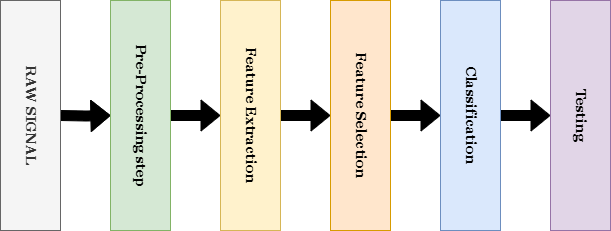
\includegraphics[width=1\linewidth]{Diagrams/icbmintro.drawio.png}
    \caption{System Architecture}
    \label{fig:sysarch}
\end{figure}
The above diagram ~\ref{fig:sysarch} shows the overall system architecture. The flow contains 6 steps (1) Data Acquisition using microphones $\rightarrow$ Raw Signal, (2) Pre-processing, (3) Feature Extraction, (4) Feature Selection, (5) Classification $\rightarrow$ SVM, (6) Testing and Validation.
The rest of this report is organized as follows. Section~\ref{sec:daq} describes the data acquisition setup and recording protocol. Section~\ref{sec:preprocess} summarizes the preprocessing steps used prior to decomposition. Section~\ref{sec:emd} presents the EMD algorithm and criteria for IMF selection. Section~\ref{sec:features} outlines the feature extraction and selection methods, and Section~\ref{sec:classification} describes the classification strategy. Experimental results and analysis are reported in Section~\ref{sec:results}, followed by conclusions and directions for future work in Section~\ref{sec:conclusion}. The DAQ setup and specific implementation details follow the experimental design in \cite{Verma2016}.

\section{Data Acquisition (DAQ) System}
\label{sec:daq}

This study used acoustic recordings to capture machine condition signatures. The DAQ choices focused on reproducibility and on maximizing signal quality while keeping the setup simple.

\subsection{Hardware and placement}
\begin{itemize}
  \item \textbf{Microphones:} Unidirectional microphones were used to preferentially pick up sound directed toward each sensor and to reduce off-axis ambient noise.
  \item \textbf{DAQ hardware:} Recordings were acquired using a National Instruments NI-9234 dynamic signal acquisition module (four channels, 24-bit) connected via an NI-9172 chassis to a PC running LabVIEW for capture and storage. This setup allows up to four simultaneous microphone channels at high sample rates.
  \item \textbf{Sensor distance:} Empirical tests showed the cleanest and loudest captures when the microphone was placed approximately 1.5 cm from the machine surface; this distance was used consistently for all recordings.
\end{itemize}

\subsection{Recording protocol}
\begin{itemize}
  \item \textbf{Duration \& sampling:} Each recording is 5 seconds long sampled at 50 kHz and stored as 24-bit PCM. Thus each raw file contains 250,000 samples.
  \item \textbf{Candidate positions:} To perform Sensitive Position Analysis (SPA) the machine was sampled at multiple candidate locations (the original study used 24 positions) so that a robust ranking of sensor positions could be obtained.
  \item \textbf{Repetitions:} Multiple (e.g., 10--20) recordings per position were acquired to enable averaging of metrics across repeats and to reduce the effect of transient disturbances.
\end{itemize}

\subsection{Practical notes and preprocessing hints}
\begin{itemize}
  \item \textbf{Useful bandwidth:} For this compressor the informative acoustic content lies largely below 12 kHz; accordingly, later processing uses a low-pass cutoff around 12 kHz and a high-pass ``fan'' filter near 400 Hz to remove known background hums.
  \item \textbf{Clipping/segmentation:} Each 5 s recording is split into 1 s segments with 50\% overlap; the segment with minimum standard deviation is selected for analysis to avoid transient spikes and to choose the most stable portion of the recording.
  \item \textbf{Smoothing \& normalization:} A simple moving-average smoother removes impulsive outliers, and a robust min–max style normalization (ignore 0.025\% extreme samples at both tails when computing min/max) is used so that scaling is not driven by rare outliers.
  \item \textbf{Storage \& labeling:} Store raw .dat (24-bit PCM) files with metadata (position ID, run number, pressure/operating point, date/time) to ensure traceability during SPA and later classification stages.
\end{itemize}

\begin{figure}[ht]
  \centering
  \fbox{\parbox{0.92\linewidth}{\centering PLACEHOLDER: schematic of DAQ (microphone positions + NI-9234) or a representative spectrogram. See Verma \textit{et~al.} (2016) for the original images.}}
  \caption{DAQ schematic and example pre-processed spectrogram (placeholder).}
  \label{fig:daq_placeholder}
\end{figure}

\subsection{Preliminary observations}
Practical tests revealed:
\begin{itemize}
    \item Microphones placed at roughly \SI{1.5}{cm} from the machine provided stronger signals and reduced background contamination.
    \item Acoustic useful content predominantly lies below \SI{12}{kHz} for the compressor under study \cite{Verma2016}; therefore, pre-processing included a high-pass filter (to remove fan hum) and a low-pass filter at \SI{12}{kHz}.
    \item A clipping strategy (segment selection) with overlap helps to choose the most stable portion of each recording for robust analysis (detailed in Section~\ref{sec:preprocess}).
\end{itemize}

% \section{Pre-processing highlights}
% \label{sec:preprocess}
% Before applying EMD, a set of standard pre-processing operations is applied to reduce sensor artifacts and outliers:
% \begin{enumerate}
%     \item \textbf{Filtering:} Remove low-frequency ambient noise (fan hum) with a high-pass filter (cutoff $\sim 400\,$Hz) and suppress very high-frequency noise using an 18th-order Butterworth low-pass with cutoff at \SI{12}{kHz} \cite{Verma2016}.
%     \item \textbf{Clipping:} Divide the 5-second signal into overlapping 1-second windows (50\% overlap) and pick the window with minimum standard deviation to avoid transient disturbances.
%     \item \textbf{Smoothing:} Apply a moving-average filter to suppress impulsive outliers while preserving important oscillations.
%     \item \textbf{Normalization:} Use a robust min--max style scaling that discards extreme 0.025\% samples at both tails (an implementation-friendly histogram-binning algorithm was proposed in \cite{Verma2016}).
% \end{enumerate}

% A schematic of the overall processing pipeline is shown in Fig.~\ref{fig:pipeline} (this is a placeholder; you should replace the placeholder with a real spectrogram or sample waveform from your data).

% \begin{figure}[H]
%     \centering
%     \fbox{\parbox{0.85\linewidth}{\centering PLACEHOLDER: Insert pre-processing pipeline figure or a sample spectrogram here (see Fig. 5 in \cite{Verma2016}).}}
%     \caption{Pre-processing pipeline: filtering, clipping, smoothing and normalization produce a ready signal for EMD.}
%     \label{fig:pipeline}
% \end{figure}

% \section{Mathematical preliminaries}
% \label{sec:formulas}
% This section collects the essential formulae used in the algorithms.

% \subsection{Empirical Mode Decomposition (EMD)}
% EMD is an iterative sifting process that extracts IMFs. In a shorthand notation, let \(x(t)\) be the input signal. The first sift produces a detail signal \(h_1(t)\) by subtracting the local mean:
% \[
% m_1(t) = \frac{e_{\text{upper}}(t) + e_{\text{lower}}(t)}{2}, \qquad
% h_1(t) = x(t) - m_1(t).
% \]
% If \(h_1(t)\) does not satisfy the IMF conditions (zero-mean envelope and extrema vs zero-crossing parity), the sifting repeats on \(h_1\):
% \[
% h_{1k}(t) = h_{1(k-1)}(t) - m_{1k}(t),
% \]
% until convergence. When convergence is reached, the last \(h_{1k}(t)\) is designated IMF\(_1\). The residue is then \(r_1(t)=x(t)-\text{IMF}_1(t)\) and the process continues on \(r_1(t)\) to extract subsequent IMFs:
% \[
% x(t) = \sum_{i=1}^n \text{IMF}_i(t) + r_n(t).
% \]

% A common stopping criterion for each IMF's sifting loop is:
% \begin{itemize}
%     \item the number of zero-crossings and extrema differ at most by one, and
%     \item the sum-of-difference (SD) between successive sifted signals drops below a small threshold \(\varepsilon\) (the source used \(\varepsilon=0.1\) as an empirical choice).
% \end{itemize}

% \subsection{Hilbert transform and envelope}
% Given a real signal \(x(t)\), its Hilbert transform \(\mathcal{H}\{x\}(t)\) is
% \[
% \mathcal{H}\{x\}(t) = \frac{1}{\pi}\, \mathrm{P.V.} \int_{-\infty}^{\infty} \frac{x(\tau)}{t-\tau}\, d\tau,
% \]
% where P.V. denotes the Cauchy principal value. The analytic signal is
% \[
% z(t) = x(t) + j\,\mathcal{H}\{x\}(t).
% \]
% Instantaneous amplitude (the envelope) and instantaneous phase are:
% \[
% A(t) = |z(t)| = \sqrt{x(t)^2 + \mathcal{H}\{x\}(t)^2},\qquad
% \phi(t) = \arg z(t) = \arctan\!\bigg(\frac{\mathcal{H}\{x\}(t)}{x(t)}\bigg).
% \]
% The envelope \(A(t)\) is used to compute positional statistics (RMS and absolute mean) in SPA.

% \subsection{Discrete Fourier Transform (DFT)}
% For completeness, the DFT of a discrete-time signal \(x[n]\) of length \(N\) is
% \[
% X[k] = \sum_{n=0}^{N-1} x[n] e^{-j 2\pi k n / N}, \qquad k=0,\ldots,N-1.
% \]

% \section{Algorithm 1: EMD sifting (flowchart)}
% \label{sec:alg1}

% \begin{figure}[H]
% \centering
% \begin{tikzpicture}[node distance=10mm]
% \node (start) [startstop] {Start: input signal $x(t)$};
% \node (findext) [process, below=of start] {Find local maxima/minima of current signal};
% \node (envelopes) [process, below=of findext] {Interpolate maxima/minima to get upper/lower envelopes};
% \node (mean) [process, below=of envelopes] {Compute mean $m(t) = (e_{\text{upper}}+e_{\text{lower}})/2$};
% \node (subtract) [process, below=of mean] {Compute detail $h(t) = \text{signal} - m(t)$};
% \node (stopcrit) [decision, below=of subtract, aspect=2] {IMF conditions met?\\(zero crossings/extrema parity and SD$<\varepsilon$)};
% \node (saveimf) [process, below=of stopcrit, yshift=-6mm] {Save $h(t)$ as IMF$_i$; compute residue $r(t)=\text{signal}-\text{IMF}_i$};
% \node (continue) [decision, below=of saveimf, aspect=2] {Residue has extrema?};
% \node (end) [startstop, below=of continue] {Stop: output IMFs and residue};

% \draw [arrow] (start) -- (findext);
% \draw [arrow] (findext) -- (envelopes);
% \draw [arrow] (envelopes) -- (mean);
% \draw [arrow] (mean) -- (subtract);
% \draw [arrow] (subtract) -- (stopcrit);
% \draw [arrow] (stopcrit) -- node[right]{No} (findext);
% \draw [arrow] (stopcrit) -- node[right]{Yes} (saveimf);
% \draw [arrow] (saveimf) -- (continue);
% \draw [arrow] (continue) -- node[right]{Yes} (findext);
% \draw [arrow] (continue) -- node[right]{No} (end);
% \end{tikzpicture}
% \caption{Algorithm 1: EMD sifting process for extracting IMFs.}
% \label{fig:alg1}
% \end{figure}

% \section{Algorithm 2: EMD-based SPA ranking (flowchart)}
% \label{sec:alg2}

% \begin{figure}[H]
% \centering
% \begin{tikzpicture}[node distance=10mm]
% \node (start) [startstop] {Start: recordings from multiple candidate positions};
% \node (pre) [process, below=of start] {Preprocess each recording (filter, clip, smooth, normalize)};
% \node (emdproc) [process, below=of pre] {Decompose preprocessed recording into IMFs using Algorithm 1};
% \node (corr) [process, below=of emdproc] {Compute correlation of each IMF with original recording};
% \node (select) [process, below=of corr] {Select IMFs with correlation $>$ threshold $\tau$ (relevant IMFs)};
% \node (recon) [process, below=of select] {Reconstruct signal using selected IMFs: $\hat{x}(t)=\sum_{j\in S}\text{IMF}_j(t)$};
% \node (hilb) [process, below=of recon] {Compute envelope via Hilbert transform: $A(t)=| \hat{x}(t)+j\mathcal{H}\{\hat{x}\}(t)|$};
% \node (stats) [process, below=of hilb] {Compute RMS and absolute mean of envelope; average across recordings};
% \node (rank) [process, below=of stats] {Rank positions by combined statistic (sum of ranks) };
% \node (end2) [startstop, below=of rank] {Stop: choose highest-ranked sensitive position(s)};

% \draw [arrow] (start) -- (pre);
% \draw [arrow] (pre) -- (emdproc);
% \draw [arrow] (emdproc) -- (corr);
% \draw [arrow] (corr) -- (select);
% \draw [arrow] (select) -- (recon);
% \draw [arrow] (recon) -- (hilb);
% \draw [arrow] (hilb) -- (stats);
% \draw [arrow] (stats) -- (rank);
% \draw [arrow] (rank) -- (end2);
% \end{tikzpicture}
% \caption{Algorithm 2: Ranking sensor positions using EMD-based reconstruction and Hilbert-envelope statistics.}
% \label{fig:alg2}
% \end{figure}

% \section{Implementation notes and practical choices}
% \begin{itemize}
%     \item \textbf{Correlation threshold \(\tau\):} The source study empirically chose \(\tau\) by analyzing many IMFs across recordings; you should choose \(\tau\) by inspecting correlation histograms for a pilot dataset.
%     \item \textbf{Number of recordings per position:} Collect multiple (e.g., 10--20) 5-second recordings per candidate position and average the RMS/mean envelope metrics across them for robust ranking.
%     \item \textbf{Computational cost:} EMD is iterative and can be expensive for long signals or many recordings. Consider segmenting the data or using fast EMD variants if computation time is an issue.
%     \item \textbf{Envelope stats:} Use RMS and absolute mean as in \cite{Verma2016}; other descriptors (median amplitude, percentiles) can be added if needed.
% \end{itemize}

% \section{Placeholders for the remaining report sections}
% Below are recommended section headers you can fill in to reach a full ~10 page report. I have provided short prompts you can expand.

% \subsection*{Results (suggested content)}
% \begin{itemize}
%     \item Present sensor position rankings (table) and final chosen position.
%     \item Show representative raw vs reconstructed signals and their envelopes (figures).
%     \item Compare SPA rankings with and without EMD (demonstrate improved consistency).
% \end{itemize}

% \subsection*{Feature extraction and selection}
% Explain time-domain, frequency-domain, and time-frequency features (FFT bins, wavelet packet energies, etc.) and the dimensionality reduction methods you use (mRMR, NMIFS, PCA), as discussed in \cite{Verma2016}.

% \subsection*{Classification and evaluation}
% Describe SVM multiclass decomposition strategies (OAO, OAA, DDAG) and cross-validation details used to evaluate the full diagnosis pipeline.

% \subsection*{Discussion}
% Discuss strengths, limitations, computational trade-offs, and potential extensions (adaptive online models, multiple-fault recognition).

% \subsection*{Conclusion}
% Summarize findings and practical recommendations.

% \section*{Example table: sensor ranking (format)}
% \begin{table}[H]
% \centering
% \caption{Example ranking table layout for sensor positions (fill with experiment data).}
% \label{tab:ranking}
% \begin{tabular}{cccccc}
% \toprule
% Position & Avg RMS (env) & RMS Rank & Avg AbsMean (env) & AbsMean Rank & Sum of Ranks \\
% \midrule
% 1 & 0.123 & 5 & 0.045 & 6 & 11 \\
% 2 & 0.242 & 1 & 0.112 & 2 & 3 \\
% 8 & 0.238 & 2 & 0.118 & 1 & 3 \\
% \bottomrule
% \end{tabular}
% \end{table}

\section*{References}
\begin{thebibliography}{1}
\bibitem{Verma2016}
N.~K. Verma, R.~K. Sevakula, S.~Dixit, and A.~Salour, ``Intelligent condition based monitoring using acoustic signals for air compressors,'' \emph{IEEE Transactions on Reliability}, vol.~65, no.~1, pp. 291--307, Mar. 2016. doi:10.1109/TR.2015.2459684.
\end{thebibliography}

\end{document}
